\documentclass[aps,prb,twocolumn,groupedaddress,nofootinbib,floatfix]{revtex4}
%
\usepackage{graphicx} 
\usepackage{graphics}
\usepackage{caption}
\usepackage{subcaption}
\captionsetup{compatibility=false}
\usepackage{amsmath}
\usepackage{bm}

%\setlength{\skip\footins}{0.3in}
\begin{document}
%
\title{Migration and Segregation in Three Dimensional Cellular Co-cultures: Role of
Differential Cell Adhesion and Elasticity}

%
\author{Daniel Kolbman}
%
% DON'T CHANGE ANYTHING IN THE NEXT FEW LINES OR DELETE BLANK LINES
%
\affiliation{This work was submitted as part of a course requirement for completion of the BS degree in the Physics Program at RIT and, in its current form, does not appear in any publication external to RIT.}
% % PUT YOUR ADVISOR NAME BELOW.  DON'T DELETE ANY LINES
%
\altaffiliation [Rochester Institute of Technology, School of Physics and Astronomy, Faculty Advisor: ]{Moumita Das}

\date{\today}

\begin{abstract} \noindent The biophysics of cell co-cultures, i.e. a binary system of cell populations, is of great interest in many biological processes including formation of embryos, and tumor progression. 
During these processes, different types of cells with different physical properties are mixed with each other, with important consequences for cell-cell interaction, aggregation, and migration. 
Until recently, experiments and theoretical models of cell co-cultures have focused on two dimensional systems. Under physiological conditions, however, cells often have to  
navigate three dimensional and confined micro environments. We will model such cell co-culture systems by extending previous two-dimensional Brownian Dynamics simulation of a binary system of interacting, 
active, and deformable particles to a confined three-dimensional system. Our results will be compared with ongoing experiments done by our collaborators. Our results may 
provide insights into the role of the difference in physical properties such as cell elasticity, cell-cell adhesion, and cell self-propulsion speeds of two cell types in emergent collective properties 
such as cell aggregation and differential migration experimentally observed in co-cultures of breast cancer cells and healthy breast epithelial cells.  

\end{abstract}

\maketitle

\section{Background and Motivation}

In several biological processes, from the formation of embryos to the formation and progression of tumors, cells with different physical properties are present in close proximity, with important
consequences for cell-cell interaction, aggregation, and migration. Laboratory cell co-cultures made of two different cell populations are ideal systems to qualitatively and quantitatively 
study how distinct physical properties of cells can influence such emergent behavior. Here we construct and study a simple proof of concept model of a cell co-culture in three dimensions 
and under confinement to test the hypothesis that differential physical properties of cells can drive segregation and preferential migration in co-cultures.   
The experimental system that motivates our work is a co-culture of breast cancer cells and non-cancerous breast epithelial cells. 
This system provides an excellent platform because of the characteristic differences between the two cell types \cite{Lee,Mingming}. 
The nucleus and cytoplasm of breast cancer cells have been found to have relatively low elastic moduli compared to their non-cancerous counterparts \cite{Lee}. 
As a result, the cancer cells are much more deformable. Recent experiments suggest that this mechanical mismatch may play a key role in cancer cell migration through a healthy
cell population \cite{Lee}. 

Until recently, most experiments and models of cell co-cultures have focused on two dimensional systems, with limited application to physiological conditions\cite{Jong}.
Recently, new techniques for observing co-cultures in three dimensions have become available\citep{Alessandri}.
Accordingly, we seek to formulate a minimal model of co-culture cell mechanics in three dimensions by extending previous two dimensional simulations of binary systems of deformable and active colloids\cite{Butcher}.
Together with our experimental collaborators Drs Wu and Ma at Cornell university, we aim to characterize the role of difference in physical properties such as cell stiffness, cell-cell adhesion, and self-propulsion in aggregation and migration in co-cultures of breast cancer cells and non-cancerous cells in three dimensions.
Furthermore, we will focus on confined systems to better recreate the physiological and experimental systems we are studying.
From a physics perspective, we will study the interplay of cell mechanics, and statistical mechanical in cell migration in a confined binary system in three dimensions.
The main ingredients of the model are discussed below.\\


\subsection{Behavior of Healthy and Cancerous Cells}

Healthy and cancerous breast epithelial cells, particularly MCF-7 and MDA-MB-231, have been widely studied and their physical properties well known \cite{}.
Experimental work involving these two cell types has shown interesting behavior in co-culture systems of these breast cells.
One such behavior occurs when cancerous cells are introduced to a monolayer of healthy cells.
In this experiment, the cancer cells are observed to have higher migration rates than when in a monolayer consisting soley of other cancerous cells \cite{Lee}.
Another interesting behavior obsered by experimentalists is the separation of the two cell types.
When a co-culture of cancerous and healthy cells are confined in a spherical droplet, they are seen to separate with cancerous cells gathering around the boundaries of the droplet and the healthy cells aggregating in the center \cite{Mingming}.

%In addition to the difference in stiffness \cite{Lee}, the adhesion properties of cancer cells have also been found to be drastically different from that of non-cancerous cells\cite{Jeanes}.
%Most healthy cells adhere to each other via the protein E-cadherin when they come in contact \cite{Suresh}. Cancer cells lack this adhesiveness.
%Cancer cells further show enhanced self-propulsion (i.e. how fast individual cells can propel themselves by consuming ATP or due to other internal forces in the absence of any other interaction forces), compared to non-cancerous cells of the same tissue type. The differences in the adhesiveness, stiffness, and self propulsion of the two cell types is a key ingredient in our model.\\
\\

\subsection{Cell Migration in Three Dimensions}

Previously several experimental and theoretical studies have addressed various aspects of cell migration in two dimensions, including protrusion, adhesion, and retraction at the level of single cells, and collective motion at the multicellular level \cite{}.
However, the {\it in vivo} environment for a crawling cell is typically a three-dimensional environment, consisting of the extracellular matrix (ECM) and surrounding cells.
Recent experiments show increased migration rates of cells in three-dimensional matrices as opposed to two-dimensional surfaces \cite{Cukierman}.

\subsection{Role of Confinement}

Ongoing experiments in the laboratories of our collaborators Dr. M. Wu and Dr. M. Ma involve observing co-cultures inside spherical capsules with diameters of the order of several hundred micro-meters 
and containing hundreds of cells\cite{Alessandri} (See FIG. \ref{fig:capsule}). Given that confinement and finite system size can have important consequences for the statistical mechanics and collective 
properties of the cell-culture, it will be vital to account for them in our model. The spherical capsules in the experiments we will model have an inner diameter of $50-700$ micro-meters and an outer diameter of $400-7000$ micro-meters.
The cells are present inside the inner capsule and have a dimensions of the order of $\sim 10$ micro-meters. The region between the inner and outer diameters is occupied by a dense gel layer that the cells can not penetrate.
The outside of this layer is coated such that cells will not adhere to this layer upon contact. \\

\begin{figure}
  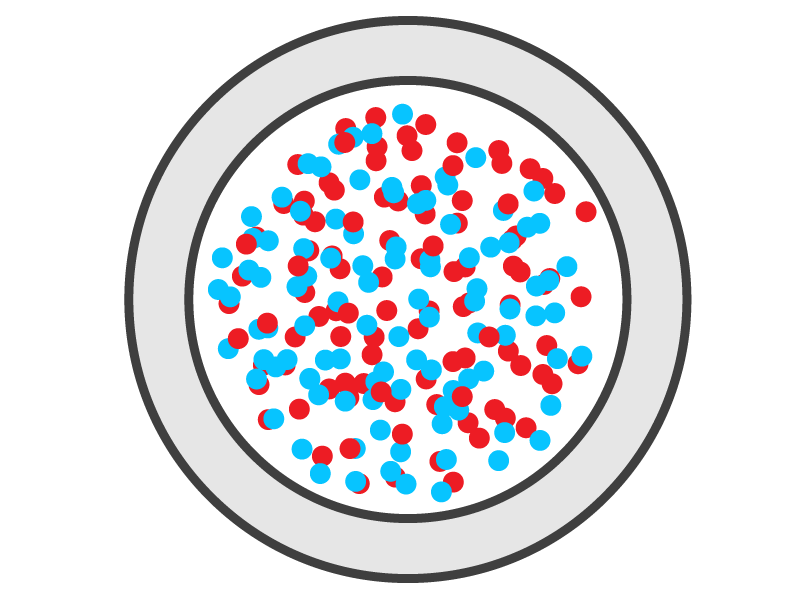
\includegraphics[width=3in]{Fig1.png}
  \caption[capsule]
   {A cross section of a spherical capsule enclosing a binary mixture of 
   cells.}
   \label{fig:capsule}
\end{figure}


\section*{Model}

\begin{figure}
  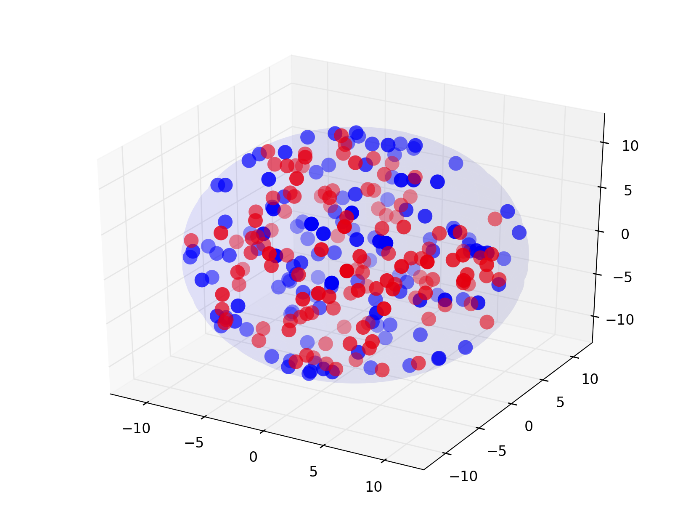
\includegraphics[width=1.0\columnwidth]{3dconf.png}
  \caption[3dconf]
    {A sample configuration of a confined three dimensional co-culture system.}
   \label{fig:3dconf}
\end{figure}

We study the collective dynamics of this system using an active Brownian Dynamics simulation. Brownian dynamics is ideal for this system as cells behave like Brownian particles: 
their dimensions and timescale of motion are much larger than that of the particles of the surrounding medium in which they are suspended and in equilibrium  their motion is diffusive. In addition
our system is ``active" because cells can generate forces by consuming ATP and propel themselves. A simple model of homogeneous monolayers of such active particles consists
of a two dimensional system of interacting colloidal particles that are also each active, i.e. self-driven \cite{FilyMarchetti,RednerBaskaran}. 
Such models have been previously used to study swarming  behavior \cite{Vicsek} in birds, insects and fish. Our group has recently combined this approach with cell 
mechanics and applied it to a binary population of cells, to study the collective mechanics and dynamics in cell co-cultures characterized by a difference in cell stiffness.
This study found that mechanical mismatch in co-cultures can have important consequences cell migration, and can lead to enhanced motility for more deformable cells\cite{Butcher}, 
in agreement with the Lee and coworkers \cite{Lee}. In this project, we extend this model to a three-dimensional system, include cell-cell adhesion, and further add the presence of a 
confining sphere to mimic the experimental set-up used by our collaborators \cite{Mingming}. 


Our model co-culture is made of two sets of active Brownian particles representing the cells (See FIG. \ref{fig:capsule}). The cells only interact with each other when 
they come into contact. The contact interaction between cells is of two types. First, when cells come into
contact and push against each other, depending on their mechanical stiffness they will respond with different forces; this interaction is modeled as an 
elastic repulsive interaction. For the non-cancerous (stiff) cells, there further exists a cell-cell adhesion,
modeled here as an attractive interaction at contact. The cancer (comparatively soft) cells do not have this adhesion. As for non-contact forces, 
the cancer cells can generate large self-propulsion forces. The self-propulsion forces generated by non-cancerous cells are orders of magnitude smaller in comparison 
and are assumed to be zero in our model. The strengths of the interactions are tuned to mimic physiological
conditions, where we use a stiffness of 2 KPa for the stiff (healthy) cells, 0.67 KPa for the soft (cancerous) cells, and a diffusion constant of $D=1.8 \mu m^2/min$ for both cell types. 
Both cell types have the same diameter  $\sigma = 1.07$ $\mu m$.
The cancer cells are assumed to be up to ten times softer than their non-cancerous counterparts. 
Cell density is chosen to ensure a nearly confluent system. The particle positions evolve according to the over damped 
Langevin equations \cite{Lemons,RednerBaskaran,FilyMarchetti,Butcher}: 

\begin{equation}
  \bm{\dot{r}} = \frac{1}{\gamma}\bm{F}_{int}(\bm{r}) + v_p\hat{\bm{v}}_i+\sqrt{2D}\eta^T
\end{equation}

\begin{equation}
  \dot{\theta}_i=\sqrt{2D_r}\eta^R_i
\end{equation}

Where $F_{int}$ is the interaction forces on the cell from adhesion and repulsion.
The variables $\bm{r}_i$ and $\dot{\bm{r}}_i$ are the position and velocity of the i\textit{th} particle, respectively.
The constant $\gamma$ is the damping coefficient of the fluid used. It is related to the
diffusion constant, $D$, by $D=\frac{k_BT}{\gamma}$, where $k_B$ is the Boltzman constant and $T$ is temperature and has been set to $298$ Kelvin. 
The variable $v_p$ is the magnitude of propulsion and $\bm{\hat{v}}_i$ is the direction of propulsion, $\bm{\hat{v}}=(cos\theta_i, sin\theta_i)$.
The noise $\eta^T$ represents fluctuations in translational motion and account for collisions with smaller fluid particles, while
$\eta^R$ is the rotational noise to simulate fluctuations in the direction of travel from ATP use by cells. 
Both types of noise follow the fluctuation dissipation theorem:

\begin{equation}
\left\langle \eta(t)\eta(t')\right\rangle = 0 
\end{equation}
\begin{equation}
\left\langle \eta(t)\eta(t')\right\rangle = 2k_bT\gamma
\delta(t-t')
\end{equation}

% Dimension stuff %

We define $k_BT$ and $\sigma$ to be our units of energy and length and define 
unit time as $\tau = \frac{\sigma^2}{D}$. These units are respectively used to non-dimensionalize 
energy, length, and time scales in the simulation. 

% Interaction forces %

The interaction forces are important for investigating how the elasticity and adhesivity of cells affects their migration and segregation. For non-cancerous cells, 
we have modeled the stiffness of the cells using a simple Hookean spring force while we use a `V' well to model the adhesion (See FIG. \ref{fig:interaction}). 
The result is particles that will desire to be close together, while resisting overlap. Cancer cells have qualitatively similar (but weaker) elastic repulsion, and not do not show 
cell-cell adhesion because of the lack of the protein E-cadherin \cite{Jeanes}. For two cells whose centers are separated by a distance $r$, the magnitude of the repulsive and adhesive forces are:

\begin{equation}
  F_{rep}(r) = F^0_{rep} \left\{ 
    \begin{array}{lr}
      1-\frac{r}{\sigma} &, r < 0\\
      0 &, r \ge \sigma
    \end{array}
  \right.
  \label{eq:frep}
\end{equation}

\begin{equation}
  F_{adh}(r) =F^0_{adh} \left\{
    \begin{array}{lr}
      0 &, r \le \sigma \\
      \frac{|r - (\sigma+\epsilon)|}{\epsilon}-1 &, \sigma < r < \sigma+2\epsilon
    \end{array}
  \right.
  \label{eq:fadh}
\end{equation}

The amplitudes of the interaction forces are chosen depending on the species of the particle. We denote these as $F^0_{rep}$ and $F^0_{adh}$ for the repulsive and adhesive prefactors, respectively.
The forces act along the separation between the center of the two particles. 
The parameter $\epsilon$ is the phenomenological lengthscale over which the non-cancerous cells show cell-cell adhesion. 

\begin{figure}
  \begin{subfigure}{\columnwidth}
    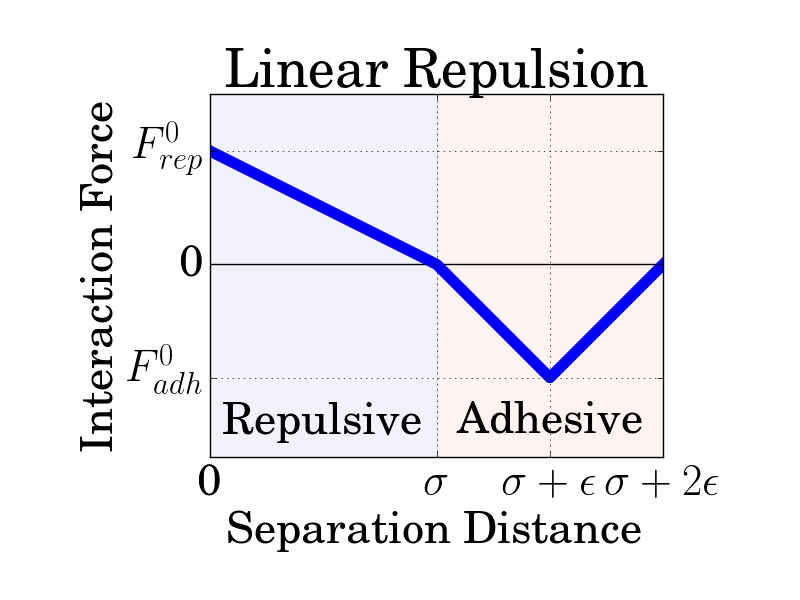
\includegraphics[width=1.0\columnwidth]{interaction.png}
  \end{subfigure}
  \begin{subfigure}{\columnwidth}
    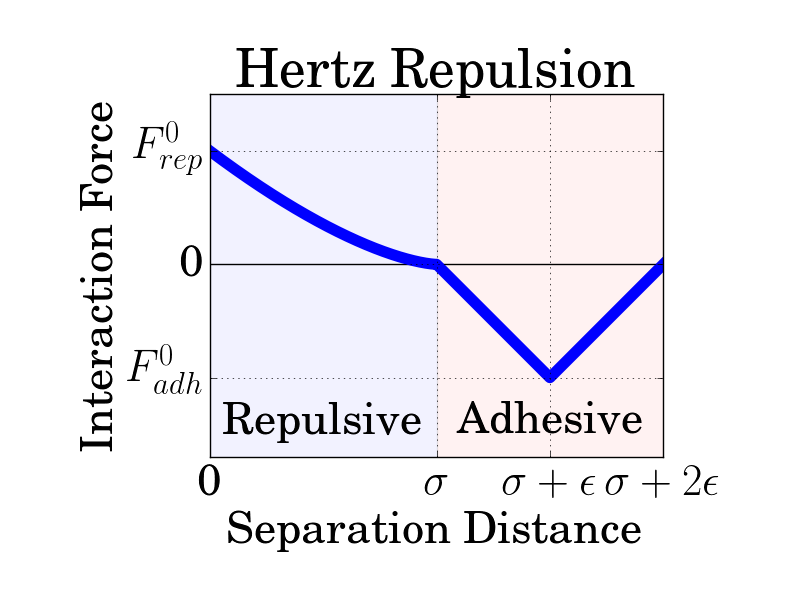
\includegraphics[width=1.0\columnwidth]{hertz.png}
  \end{subfigure}
  \label{fig:interaction}
  \caption[capsuleECM]{Schematics of the general form of the two part interaction force for the two models. For small separations within the diameter of the cells, there is a hookean or Hertzian, repulsive force. Neighboring cells outside, but near a given cell, experience an adhesive force. The strengths of the forces are determined by the prefactors $F_{rep}^0$ and $F_{adh}^0$ and the effective separation of the adhesive force by the contact distance, $\epsilon$  (Not illustrated to scale).}
\end{figure}

% Physical system (Boundaries, packing fraction) %

\subsection*{System Conditions}
We have imposed `hard' barrier boundaries on the system to imitate the conditions of confining microfluidic shells used in the experiments \cite{Mingming}. 
This means that particles may move along or within a specified radius, but are restricted from moving outside of it. We begin each simulation with an initial configuration 
where the two species are intermixed and the cells are randomly and uniformly distributed inside of the confining sphere. The size of the system is dependent on the 
packing fraction of the system. For our simulations, we choose a packing fraction of $\phi=0.4$ for each cell type, which is where active colloidal systems have been 
studied in the past\cite{RednerBaskaran}, and found to form a nearly confluent system at long times. See FIG. \ref{fig:3dconf} for a sample three dimensional system.


% Technical stuff %
\section{Numerical Methods}

The dynamics simulations are computed in Julia, a high-performance, dynamic 
programming language for scientific computing. Spatial cell hashing and neighbor 
checking was used for broad phase collision detection to linearize run times 
as a function of the number of total particles. The simulations use a foreward 
Euler method to integrate with time steps between $10^{-4}\tau$ and $10^{-6}\tau$.
Ten identical runs, reach for a different random initial configuration of cells, were run in parallel for each simulation
and averaged together to produce Mean Square Displacement (MSD) data for a given set of parameters.

\section{Results}

\subsection{Brownian Diffusion}
According to Einstein's theory of brownian motion, it is expected that the mean
square displacement of a particle undergoing Brownian motion in three dimensions should evolve proportional to the time, with a proportionality constant $6 D$, where $D$ is the diffusion constant. In our non-dimensionalized model, this constant pre-actor should be $6$. We used this fact to confirm that the dynamics of the simulation were working properly. To test this, all interaction and propulsive forces were turned off and the system was evolved only under brownian forces. Ten identical simulations were run and averaged to produce FIG. \ref{fig:brownianMSD}. The slope is very nearly the expected value and will be exact for larger numbers of trial runs and larger system sizes.

\begin{figure}
  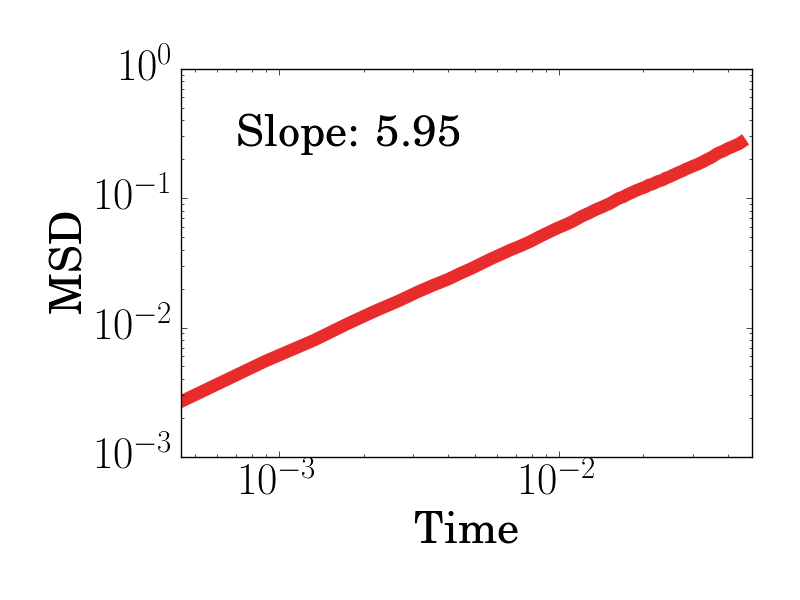
\includegraphics[width=\columnwidth]{brownianMSD.png}
  \caption[brownianMSD]
    {MSD for a single species system under only brownian forces. The MSD evolves nearly as $6Dt$ as expected from Einstein's theory of brownian motion. The time is expressed in units of $\tau$, and MSD is expressed
    in units of $\sigma^2$ defined earlier.}
  \label{fig:brownianMSD}
\end{figure}

\subsection{Segregation}

Next we focused on the segregation of the cancer cells from the non cancer cells
observed in ongoing experiments by our collaborators Drs. Ma and Wu. 
They have found that, starting with a randomly distributed mixture of breast cancer cells,
and non-cancerous breast epithelial cells inside the spherical microfluidic capsule, over long times
(of the order of weeks), the two cell types phase separate. The healthy cells assemble in the the center of capsule,
while the cancerous cells collect near the boundary and form an outer shell. By using parameters similar to those 
in the experiments, we are able to qualitatively replicate this using our model.

\begin{figure*}
  \centering
  \begin{subfigure}[t]{1.0\textwidth}
    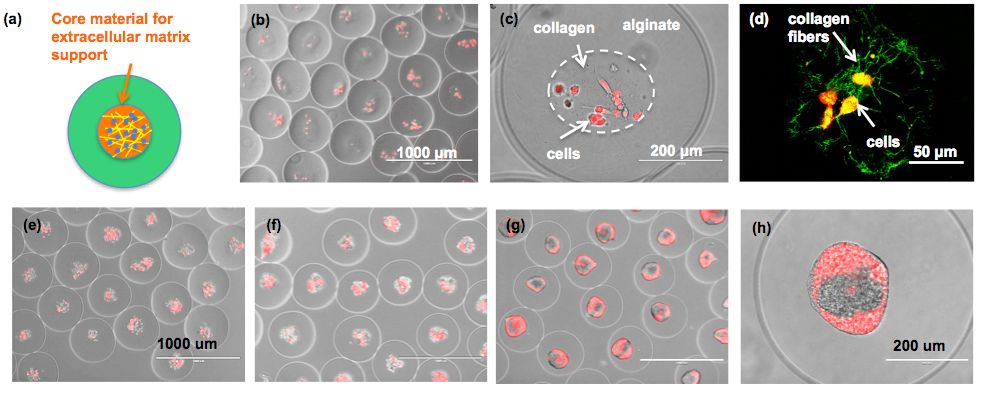
\includegraphics[width=\textwidth]{experimental.png}
  \end{subfigure}
  \begin{subfigure}[t]{1.0\textwidth}
    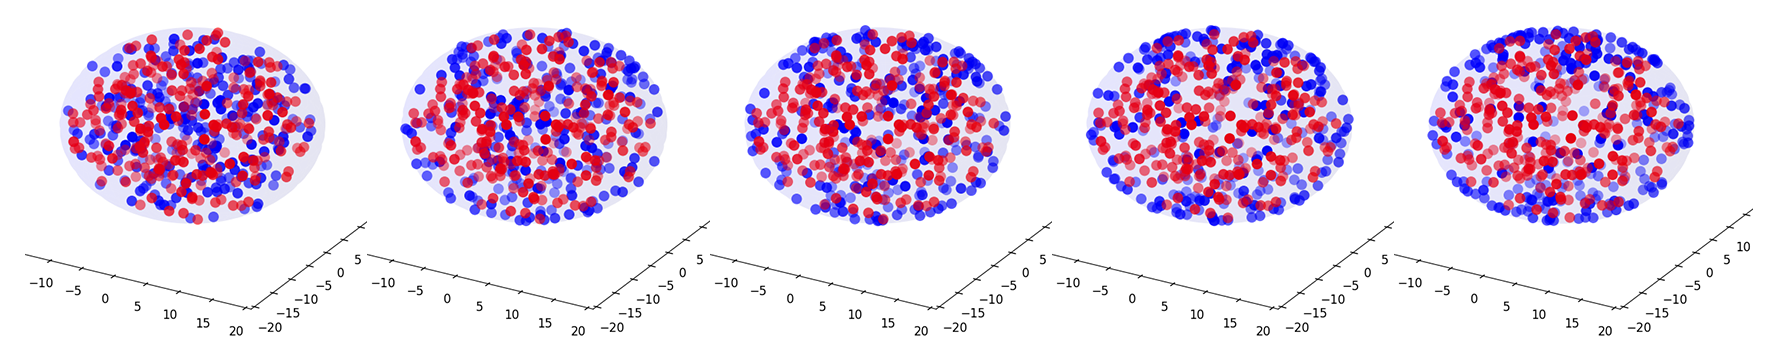
\includegraphics[width=\textwidth]{separation.png}
  \end{subfigure}
  \caption[separation]{Time evolution of the co-culture model of the cancer cells (Blue) and the healthy cells (Red) over a timescale of the order of seconds. The system evolves (left to right) from an initial, random state (left) towards a segregated state (right).}
   \label{fig:separation}
\end{figure}

We start with an initial random and uniform distribution of the two cells types consisting of  
equal number of cells for each type. As described before, the cancer cells experience an elastic
repulsion that is ten times weaker than that experience by the non-cancerous cells. Furthermore, 
cancer cells experience a self-propulsive force but no cell-cell adhesion, while non-cancerous cells
experience cell-cell adhesion, but no self-propulsion. There is no cell-cell adhesion between cancer cells
and non-cancerous cells.  Under these conditions, we allow the system to evolve (See
FIG. \ref{fig:separation}). The system separates from its initial (random) state
so that the cancerous cells move toward the boundary. We have only run our system for an experimental run time
corresponding to a few seconds. To be able to compare with the experiments more accurately, we will need to study evolution
of our system over an experimental timescale of the order of at least a week. This is currently underway. 

\begin{figure}
  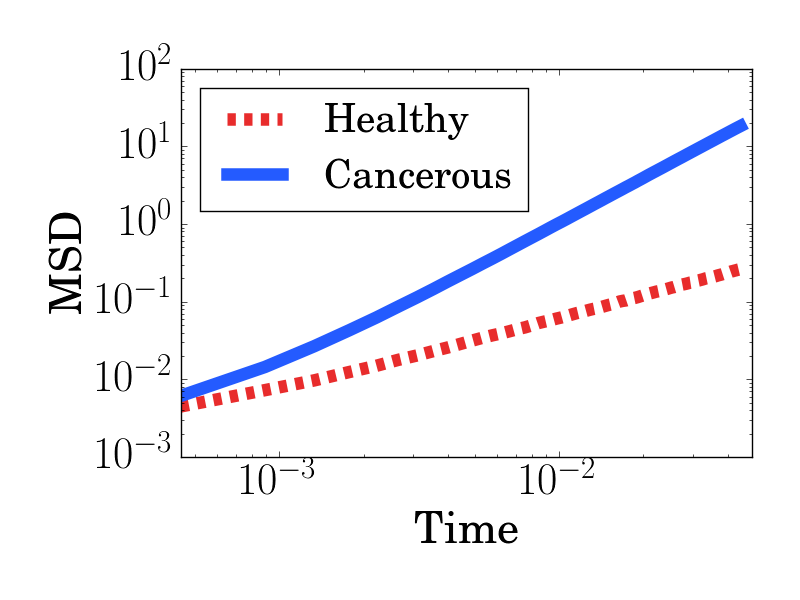
\includegraphics[width=\columnwidth]{cocultureMSD.png}
  \caption[cocultureMSD]
    {The MSD for a co-culture, cancerous-healthy cell system. The cancerous cells
    are observed to be much more motile than the healthy cells, and their MSD has a larger slope. The time is expressed in units of $\tau$, and MSD is expressed
    in units of $\sigma^2$ defined earlier. This result is
    similiar to those of the two dimensional case\cite{Butcher}.}
  \label{fig:cocultureMSD}
\end{figure}

\subsection{Differential Migration}
One case that was investigated closely in the two-dimensional model was a co-culture system with healthy, adhesive cells, and cancerous, propulsive cells with an elasticity 
difference of one order. As in the two-dimensional case, we find that in the three dimensional co-culture, the cancerous cells migrated faster than the healthy cells. This is represented by the larger
slope of the mean square displacement (MSD) vs time, for the cancer cells compared to the healthy cells. (See FIG. \ref{fig:cocultureMSD}).

\subsection{Size Dependence}

Due to the difficulty of the simulation, a system comparable to the systems produced in the lab consisting of millions of cells is not feasable.
Instead, a much smaller system (512-1024 cells) was needed to produce results in a reasonable fashion.
I ran the model under similar conditions for different quantities of cells to determine what considerations to make when comparing my model to experimental results from colaborators.

\subsection{Packing Fraction Dependence}

The critical packing fraction for solid spheres where the system becomes jammed is $0.74$.
Given that the model consists of deformable spheres as opposed to solid spheres, it was expected that the reach a critical packing fraction obove $0.74$ and show significantly reduced motility in both species.


\subsection{Stiffness Dependence}

One motivating hypothesis behind this model was that the difference in cell elasticity caused a mismatch in motility of the two cell species.
The model was run for several different ratios of stiffness between the two cells ranging up to three orders difference between the two.

\subsection{Adhesive Dependence}

\subsection{Propulsion Dependence}



\section*{Conclusions}
We have constructed a simple proof-of-concept cell co-culture model to test the hypothesis that differences in physical properties of cells in close proximity in a co-culture can influence emergent collective properties such as migration
and segregation. Our preliminary results indicate that this is indeed true.
During the next semester we will examine the full phase diagram of this system.
We will study MSD (migration), and segregation in a multi-dimensional phase space made of three physical parameters -- ratio of stiffness of the two cell types, self-propulsion of the cancer cells, and cell-cell adhesion strength of the healthy cells.
We will work closely with our experimental colleagues to identify experimentally accessible and physiologically relevant regimes in this phase diagram.
We will also add the two more components -- the presence of the ECM and cell division -- to our model that may be important for the cell segregation and migration observed in experiments.
The ECM is an important constituent of the experimental microcapsules, and we will model it has a disordered potential  (See FIG. \ref{fig:capsuleECM}).
The drastic difference in cell division rates between cancer cells and healthy cells may be crucial to the experimentally observed collective behavior of the system over the timescales (of the order of weeks) the system is monitored, and will be included by allowing for cells to divide into two following local rules. 

\begin{figure}
  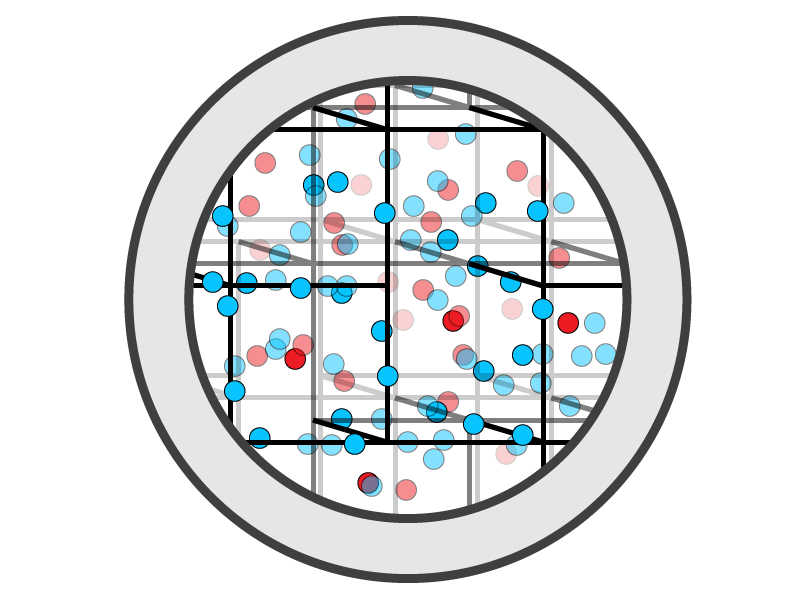
\includegraphics[width=0.9\columnwidth]{Fig2.png}
  \caption[capsuleECM]
   {A cross section of a spherical capsule enclosing a binary mixture of cells and an extracellular matrix.}
   \label{fig:capsuleECM}
\end{figure}


\section{Future Work}

\subsection{Interaction with the Extra Cellular Matrix}
The extracellular matrix (ECM) is a structural network of fibers that surrounds the cells, and interacts with the contained cells \cite{Alberts}.
Most healthy cells adhere to the ECM and move along it in a manner mimicking one-dimensional motion \cite{Cukierman}.
Migration speed of cells in this manner has been observed to be significantly higher than on two dimensional surfaces \cite{Doyle}.
Considering the ECM and the interaction of cells with the ECM will thus be very important in the development of our three-dimensional model.

\begin{acknowledgments}
Many thanks to: Dr. Moumita Das for her mentorship and inputs, Julian Butcher for useful discussions, Drs. Minglin Ma and Mingming Wu for their collaboration and discussions, 
and the Capstone Committee, especially Dr. Linda Barton, for their guidance and arranging of Capstone Program.
\end{acknowledgments}

\vspace{0.6in}
%
%change the name of the bibliography file to your own name
%make sure you have h-physrev5.bst file in the same directory as your tex file and bib file
%then compile using Latex-Bibtex-Latex-Latex sequence!
%

\bibliographystyle{h-physrev5.bst}
% now the actual bibliography file.   Note that it does not need the .bib extension in this line!
\bibliography{DanKolbmanBibliographyFile}
\end{document}

